% This is the Duke University Statistical Science LaTeX thesis template.
% It has been adapted from the Reed College LaTeX thesis template. The
% adaptation was done by Mine Cetinkaya-Rundel (MCR). Some of the comments
% that are specific to Reed College have been removed.
%
% Most of the work on the original Reed College document class and template
% was done by Sam Noble (SN). Later comments etc. by Ben Salzberg (BTS).
% Additional restructuring and APA support by Jess Youngberg (JY).
%
% See https://www.reed.edu/cis/help/latex/ for help. There are a
% great bunch of help pages there, with notes on
% getting started, bibtex, etc. Go there and read it if you're not
% already familiar with LaTeX.
%
% Any line that starts with a percent symbol is a comment.
% They won't show up in the document, and are useful for notes
% to yourself and explaining commands.
% Commenting also removes a line from the document;
% very handy for troubleshooting problems. -BTS

%%
%% Preamble
%%
% \documentclass{<something>} must begin each LaTeX document
\documentclass[12pt,twoside]{dukestatscithesis}
% Packages are extensions to the basic LaTeX functions. Whatever you
% want to typeset, there is probably a package out there for it.
% Chemistry (chemtex), screenplays, you name it.
% Check out CTAN to see: http://www.ctan.org/
%%
\usepackage{graphicx,latexsym}
\usepackage{amsmath}
\usepackage{amssymb,amsthm}
\usepackage{longtable,booktabs,setspace}
\usepackage{chemarr} %% Useful for one reaction arrow, useless if you're not a chem major
\usepackage[hyphens]{url}
% Added by CII
\usepackage{hyperref}
\usepackage{lmodern}
\usepackage{float}
\floatplacement{figure}{H}
% End of CII addition
\usepackage{rotating}

% Next line commented out by CII
%%% \usepackage{natbib}
% Comment out the natbib line above and uncomment the following two lines to use the new
% biblatex-chicago style, for Chicago A. Also make some changes at the end where the
% bibliography is included.
%\usepackage{biblatex-chicago}
%\bibliography{thesis}


% Added by CII (Thanks, Hadley!)
% Use ref for internal links
\renewcommand{\hyperref}[2][???]{\autoref{#1}}
\def\chapterautorefname{Chapter}
\def\sectionautorefname{Section}
\def\subsectionautorefname{Subsection}
% End of CII addition

% Added by CII
\usepackage{caption}
\captionsetup{width=5in}
% End of CII addition

% \usepackage{times} % other fonts are available like times, bookman, charter, palatino


% To pass between YAML and LaTeX the dollar signs are added by CII
\title{Modeling Win Probability in NFL Games}
\author{Robert Rappleye}
% The month and year that you submit your FINAL draft TO THE LIBRARY (May or December)
\date{May 2019}
\advisor{Sayan Mukherjee}
\institution{Duke University}
\degree{Bachelor of Science in Statistical Science}
\committeememberone{Alan Gelfand}
\committeemembertwo{Amy Herring}
\dus{Dus X. Name}
%If you have two advisors for some reason, you can use the following
% Uncommented out by CII
% End of CII addition

%%% Remember to use the correct department!
\department{Department of Statistical Science}

% Added by CII
%%% Copied from knitr
%% maxwidth is the original width if it's less than linewidth
%% otherwise use linewidth (to make sure the graphics do not exceed the margin)
\makeatletter
\def\maxwidth{ %
  \ifdim\Gin@nat@width>\linewidth
    \linewidth
  \else
    \Gin@nat@width
  \fi
}
\makeatother

\renewcommand{\contentsname}{Table of Contents}
% End of CII addition

\setlength{\parskip}{0pt}

% Added by CII

\providecommand{\tightlist}{%
  \setlength{\itemsep}{0pt}\setlength{\parskip}{0pt}}

\Acknowledgements{
I want to thank a few people.
}

\Dedication{
You can have a dedication here if you wish.
}

\Preface{
This is an example of a thesis setup to use the reed thesis document class
(for LaTeX) and the R bookdown package, in general.
}

\Abstract{
The preface pretty much says it all.

\par

Second paragraph of abstract starts here.
}

% End of CII addition
%%
%% End Preamble
%%
%
\begin{document}

% Everything below added by CII
  \maketitle

\frontmatter % this stuff will be roman-numbered
\pagestyle{empty} % this removes page numbers from the frontmatter
  \begin{acknowledgements}
    I want to thank a few people.
  \end{acknowledgements}
  \begin{preface}
    This is an example of a thesis setup to use the reed thesis document class
    (for LaTeX) and the R bookdown package, in general.
  \end{preface}
  \hypersetup{linkcolor=black}
  \setcounter{tocdepth}{2}
  \tableofcontents

  \listoftables

  \listoffigures
  \begin{abstract}
    The preface pretty much says it all.
    
    \par
    
    Second paragraph of abstract starts here.
  \end{abstract}
  \begin{dedication}
    You can have a dedication here if you wish.
  \end{dedication}
\mainmatter % here the regular arabic numbering starts
\pagestyle{fancyplain} % turns page numbering back on

\hypertarget{introduction}{%
\chapter*{Introduction}\label{introduction}}
\addcontentsline{toc}{chapter}{Introduction}

Predicting the winner of a given National Football League (NFL) game has long been of interest to fans, pundits and gamblers alike. Many factors can influence the outcome of a game. Some more obvious factors might include the current score differential, the amount of time left, the down, the distance to go to pick up a first down, the current yard line, and the strength of each team's offensive, defensive and special teams units. Some less obvious factors might include the number of timeouts each team has left, the stadium in which the teams are playing, the weather, which team will receive the second half kickoff, and the in-game decision making capabilities of the respective coaches.

Others have developed in-game win probability models using some of these factors. Lock \& Nettleton (2014) used a Random Forest that takes in a number of variables aimed at describing the current game state\footnote{They used down, yards to go for a first down, yard line, score differential, seconds remaining, timeouts remaining for each team, and adjusted score---score divided by the square root of seconds remaining + 1---to describe the current game state}, a variable---total points scored---that might offer insight into the level of variance associated with the game environment, and the pre-game point spread as a measure of the relative team strengths. Their model outputs the probability the team with possession of the football will win the game. Pro-Football-Reference (PFR) has published an in-game win probability model that expands on previous research by Hal Stern and Wayne Winston and treats the change in score from a given point until the end of the game as a normal distribution, calculating win probability by finding the proportion of the normal probability density function that corresponds to a final score differential that is greater than zero. A different unspecified model is used for game states where less than five minutes remain. The mean of the PFR normal distribution is taken to be the current score differential plus the expected points added (EPA), a feature designed by PFR to find the value of a given combination of down, distance to first down, yard line and time remaining in the half. The variance is taken to be 13.45\footnote{The variance of the final score from the pre-game point spread over all NFL games from 1978-2012} multiplied by the fraction of game time that remains (Paine, n.d.). Maksim Horowitz, Samuel Ventura and Ronald Yurko developed a win probability model (and the wonderful nflscrapR package that was used to load in the play by play data used in this analysis) that uses a multinomial logistic regression to evaluate the value of field position and a Generalized Additive Model (GAM) to output a win probability. ESPN also boasts a win probability model. A description of ESPN's methods was not listed on its site, but in 2017 Michael Lopez, then an assistant professor at Skidmore College, now the NFL's Director of Data and Analytics, described the model as ``derived from an ensemble of machine learning models.''

Unfortunately, of these models, only the results from the model developed by Horowitz, Ventura and Yurko (2018) are available online, though Lock and Nettleton (2014) give a summary of their model's effectiveness when tested on the 2013 NFL season and were kind enough to share the results of an updated model for games during the 2017 season. This makes it difficult to evaluate of the effectiveness of different methods or set a benchmark for what level of performance constitutes an effective model.

The aim of this work is to create a win probability model that improves upon shortcomings in existing models. Some models---Lock and Nettleton (2014), seemingly ESPN---draw upon ensemble learning methods that allow for nonlinear modeling of complex interactions, while Horowitz, Ventura and Yurko (2018) use a GAM to a similar end. Others, like PFR, draw upon the link between change in score differential and the normal distribution to utilize a known cumulative distribution function (CDF) that allows for an easy transformation to win probability space. However, no model has advertised itself as doing both\footnote{Although the lack of transparency exhibited by many of these models makes this difficult to evaluate}, a modeling process that could be carried out by modeling more granular events---the probability distribution for the outcome of a set of downs or the next scoring event, for example---in a nonlinear manner, drawing from a probability distribution that models these events and feeding the result to a normal distribution. The process of Horowitz, Ventura, and Yurko (2018) is most similar, but they substitute a GAM for a normal distribution and feed the expectation of the value of the current game state to the GAM instead of feeding samples from the distribution of future game states that might exist. Additionally, though some models may implicitly account for the possibility that games featuring different game states may feature different variances even when time remaining is held equal, no existing model appears to account for differences in variance that occur as a result of differences in the types of teams playing in one game versus another. The intuition behind this is that all else held equal, a game between two high-powered offenses would seem to feature greater variance in certain situations than one between two high powered defenses. It also stands to reason that if variance is assumed to depend on the game state and aspects of team make-up, then \(\mu\) might also. In short, this paper seeks both to flesh out some of the nuances in team composition that might affect win probability and to measure the effect of certain variables---mainly those related to field position and down and distance---indirectly through the effect that differences in distributions of future game states has on win probability.

\hypertarget{literature-review}{%
\chapter*{Literature Review}\label{literature-review}}
\addcontentsline{toc}{chapter}{Literature Review}

\textbf{Lock and Nettleton (2014)}\\
Lock and Nettleton use a Random Forest to predict game outcomes.They use many standard features to describe the game state---score differential, down, distance to first down, yard line, timeouts remaining for each team---but they added a clever feature, ``adjusted score'', where

\(adjustedScore = \sqrt{\frac{scoreDifferential}{seconds+1}}\)

This forces the model to gain a sense of the interaction between score and time remaining. Additionally, the ability of a Random Forest to find interactions between variables as well as nonlinear relationships between predictors and the response makes it a good choice for modeling win probability in NFL games. Many predictors seem to have nonlinear effects and situational interactions that are difficult to generalize. The utilization of ensemble based learning methods to help tackle this problem is one that we also used.

\textbf{Paine et al. (2019)}\\
PFR models change in score differential from the current game state until the end of the game as:

\(\Delta score \sim \mathcal{N}\)(\(\mu,\,\sigma^{2}\))~where\\
\(\mu = score\) \(differential + EPA + point\) \(spread * (seconds\) \(remaining/3600)\) and\\
\(\sigma^{2} = 13.45\)

This allows PFR to leverage the fact that any draw from this distribution that is greater than zero corresponds to a win for the team possessing the ball and any draw that is less than zero corresponds to a loss. PFR is vague about how EPA is modeled, mentioning only that it is meant to capture the ``expected average scoring consequences'' associated with the down, distance to first down, yard line and time left of the game state. Though PFR's model is relatively barebones and the page describing it does not really outline how PFR handles game states with five minutes or fewer remaining---the point at which they presume the assumption that change in score follows a normal distribution breaks down---the trick PFR uses to apply a normal distribution to the problem of win probability prediction is one that we will borrow. We also utilize a scaled point spread to help inform the \(\mu\) parameter of our normal distribution.

\textbf{Horowitz, Ventura and Yurko (2018)}\\
Win probability is modeled through a two step process in this paper. First, a multinomial logistic regression model is fitted to specify a probability distribution for the type of scoring play that will occur next given the variables: down, seconds remaining in the half, yard line, a log transform of yards to go for a first down, and indicator variables for whether the current set of downs is ``goal-to-go'', meaning the end zone is the first down marker, and whether two minutes or fewer remain in the half. The seven possible outcomes include a touchdown, field goal, or safety by the current offense, a touchdown, field goal, or safety by the current defense, or no score within the same half. The multinomial regression is computed by running a logistic regression that compares the probability of each type of scoring play to the baseline of no scoring plays for the remainder of the half and normalizes the combined results of the paired logistic regressions to find a valid probability distribution. Next, the expected value of the resulting probability distribution is added to the current score differential to produce an expected score differential. The expected score differential is plugged into a GAM, along with the timeouts remaining for each team, seconds remaining in the half, a ratio of expected score to seconds remaining, and the indicators for goal-to-go and whether two minutes or fewer remain. This GAM predicts the probability that the team possessing the ball will win the game. The decision to first predict the next scoring play before attempting to predict the overall win probability is one we intend to mirror. We will also make the choice to model the expected points added by field position as the expected value of a multinomial distribution instead of as the expected value of a continuous distribution. One quirk of the model is that it does not consider team strength when outputting predictions---each game begins with both teams possessing a 50\% chance of winning per the model. The authors actually designed this model merely to have a coherent method of calculating the expected points added or subtracted by the players on the field\footnote{The model is just one section of their paper!} and adding in team strength would ``artificially inflate (deflate) the contributions made by players on bad (good) teams'' (Horowitz, Ventura and Yurko, p.~15). As such the model is purposefully leaving a little bit on the table.

\textbf{Friedman (2001 \& 2002)}\\
Friedman's Gradient Boosting Machine works by additively fitting a succession of decision stumps to create a forest. Gradient descent is performed using a specified loss function and each successive tree is fit to minimize the loss function. The ability to specify a loss function to use in the gradient descent process allows gradient boosting to be extended to the multinomial distribution, making it a good fit for some of the multinomial classification problems that pop up in this paper. Boosting models offer many of the same advantages as the random forests used by Lock and Nettleton (2014).

\textbf{Schatz et al. (2019)}\\
Football Outsiders created a proprietary metric called Defensive-adjusted Value Over Average (DVOA) that they use to measure offensive, defensive and special teams success on a play by play basis. DVOA adjusts for context, meaning a five yard pick-up on third and four is worth more than a nine yard pick-up on third and fifteen, and uses a system of ``success points'' to evaluate plays. Teams with an offensive DVOA of ten percent are ten percent better than league average. Defensive DVOA works the opposite way---a team with a defensive DVOA of ten percent is ten percent worse than league average. DVOA is one of the most commonly used measurements of offensive, defensive and special teams caliber, hence its use in this paper.

\textbf{Eager et al. (2019)}\\
Pro Football Focus has a team of analysts that watches every play of the NFL season and assign grades to players for each play. The grades are based on a rubric before being adjusted for the difficulty level of each play (i.e.~was a quarterback being pressured when he threw or did he have a clean pocket). These grades may be subject to human error.

\textbf{Burke and Katz (2017)}\\
ESPN's Total QBR works by analyzing each play a quarterback is involved in and classifying the play as either a success or a failure. Burke and Katz then turn this classification into a score by factoring in the competitiveness of the game situation\footnote{Competitve situations are weighted more heavily.}, the quarterback's level of responsibility for the play outcome, and the level of difficulty of the play.

\hypertarget{data}{%
\chapter{Data}\label{data}}

\textbf{1.1 Description of the Play-by-Play Data}\\
The play-by-play dataset comes from the NFL JSON API courtesy of the nflscrapR package, developed by Maksim Horowitz and Ron Yurko, which gives R users the API data in an easily digestible data frame. This package was used to compile a dataset of every play from the 2010 through 2017 NFL seasons. The dataset includes a number of variables that describe the game state including down, yards to go until a first down, yard line, and seconds remaining. The dataset also contains many variables that were helpful when it came to cleaning the data and adding features, including a description of each play that uses specific and consistent verbiage for different types of plays, making it easy to use text matching to search the dataset.

\textbf{1.2 Cleaning the Data}\\
Though the nflscrapR package simplified the complexities of pulling data from the NFL JSON API and formatted it nicely in a dataframe, the actual contents of the data was still a bit raw. We matched each game to a dataset of game outcomes and pre-game point spreads\footnote{The pre-game lines were usually compiled on Sunday mornings according to the steward of the website so they will occasionally differ from the closing line} provided by The Prediction Tracker, and looked for discrepancies between the final score as listed in the play-by-play dataset and the point spread dataset. This allowed us to find games and plays in which the score was incremented incorrectly in the play-by-play dataset. We also looked for plays where the number of seconds remaining, the down or the field position changed from one play to the next in an incoherent manner to either fix or omit clearly erroneous entries.

\textbf{1.3 Incorporating Other Datasets}\\
Though the play-by-play dataset contains all the information one might need as far as describing the game state is concerned, it does not contain any information to describe the teams playing in each game. To remedy this issue we consulted several other datasets. We grabbed grades assigned to quarterbacks from 2008 through 2017 by Pro Football Focus (PFF) and pulled age, the pick at which a player was drafted, passing attempts and ESPN's Total QBR from Pro Football Reference (PFR) to use in a model that projects the grade a quarterback will receive in a given season\footnote{This model is included in the appendix}. We also downloaded the aforementioned point spreads and game outcomes from The Prediction Tracker. Lastly, we also pulled week by week Defense-adjusted Value Over Average (DVOA) ratings for offense, defense and special teams from Football Outsiders through the use of a web scraping script. Each of these descriptors of team (or player) strength was mapped to the rows of the dataset that contained the appropriate team and week match as either a ``Home Team'' descriptor or an ``Away team'' descriptor. An example of some of the predictors in the data might look something like this:
\begin{longtable}[t]{rrrrrrr}
\caption{\label{tab:sample-data}Sample Use of Outside Data}\\
\toprule
Point Spread & QB Home & QB Away & Off DVOA Home & Off DVOA Away & Def DVOA Home & Def DVOA Away\\
\midrule
-3.0 & 68.4 & 80.9 & 10.4 & 2.3 & 18.7 & 1.4\\
4.5 & 72.6 & 69.9 & 1.6 & -2.9 & 17.5 & -5.4\\
-3.0 & 62.6 & 76.9 & -17.7 & 3.9 & 0.0 & 1.6\\
-5.5 & 70.2 & 91.5 & 5.2 & 9.7 & 29.2 & 11.3\\
7.0 & 72.9 & 71.2 & 19.8 & -1.8 & -26.6 & 6.5\\
\bottomrule
\end{longtable}
Where ``QB Home'' and ``QB Away'' refer to the projected PFF grades for each team's quarterback. The point spread, is the amount the home team is favored by\footnote{Negative amounts signal that the away team is favored}. These variables are transformed to describe the ``possession team''---the team with the ball---and the defensive team when eventually used in models. Additionally, it is important to note that each value of DVOA is given a prior set to the pre-season projection of DVOA for the team in question. This prevents early season games from leading to extreme values for DVOA. The prior has a weight of four games\footnote{This prior was chosen as a sort of average of the game weights that Football Outsiders assigns to its pre-season projection prior which diminish as the season goes on and range from one to nine games}.

\textbf{1.4 Exploratory Data Analysis}\\
To get a sense of whether or not the assumption made by PFR that the change in score differential at a given point in a game is normally distributed we plot the density of change in score differential for the first five minutes of each quarter. We only sample data points from kickoffs in order to give equal weight to each unique score, game pair in each dataset.

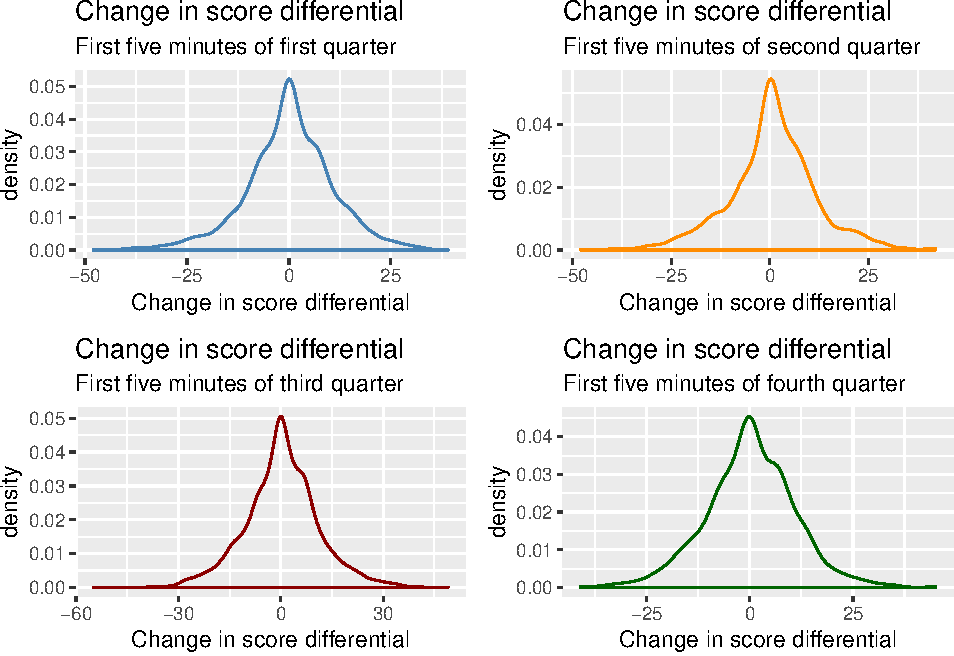
\includegraphics{thesis_files/figure-latex/normality-eda-1.pdf}

We next take a look at how the absolute value of change in score differential scales as the game goes on, again sampling only from kickoffs.This should give a sense of whether or not variance scales as the game progresses.

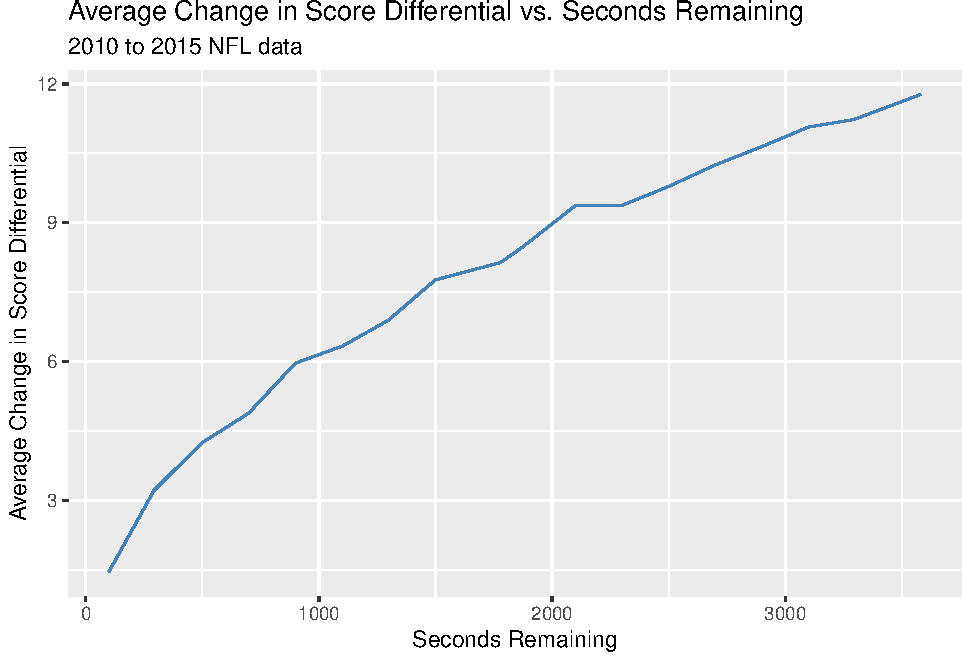
\includegraphics{thesis_files/figure-latex/variance-eda-1.pdf}

We also take a look at the probability of the next scoring play being of a given type based on the yardline the ball is currently positioned at, this time for all first down plays. This will give an idea of whether the relationship between yard line and next scoring event is linear for different events.

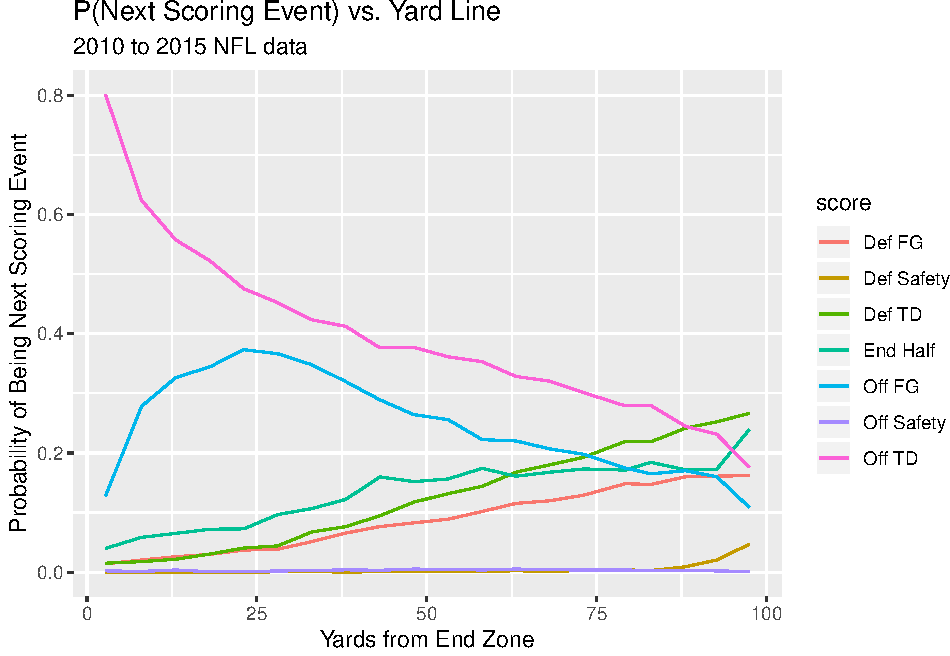
\includegraphics{thesis_files/figure-latex/scoring-plays-1.pdf}

Finally, we'll take a look at how the probability of different outcomes on a given set of downs changes with the yards to go. We'll output graphs for both first and second down.

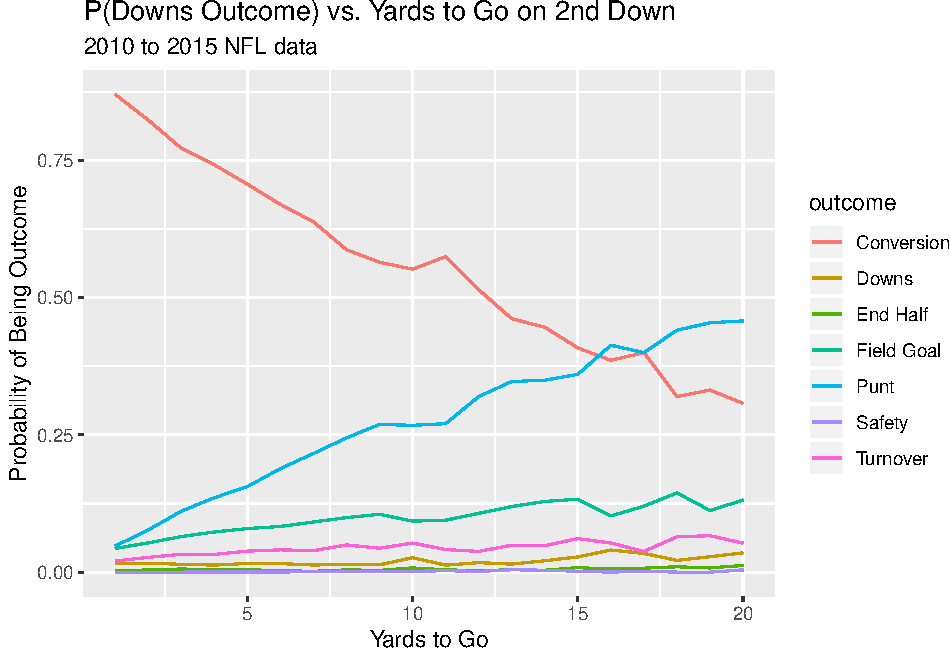
\includegraphics{thesis_files/figure-latex/downs-plays-1.pdf} 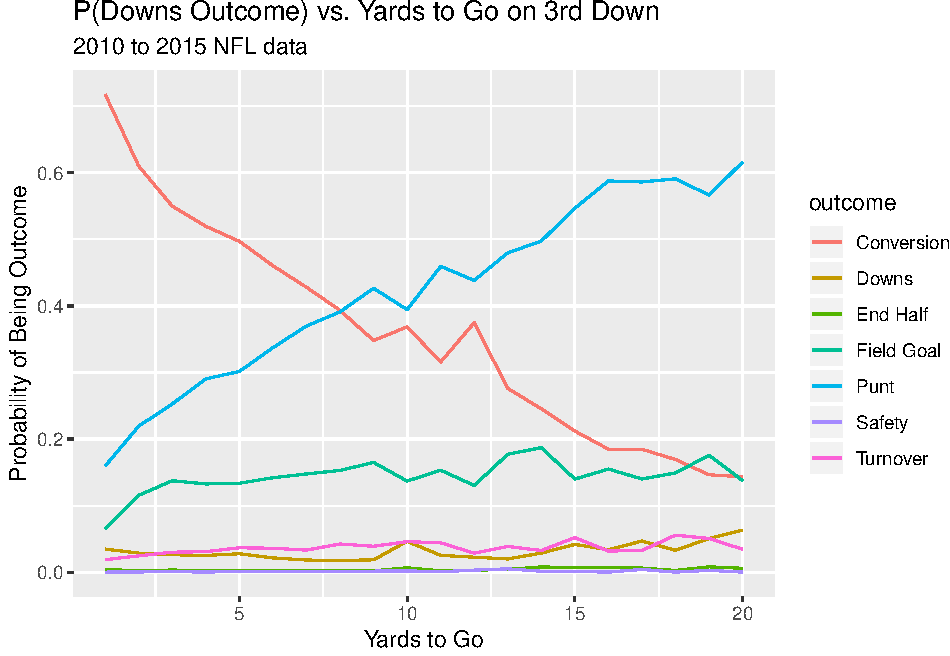
\includegraphics{thesis_files/figure-latex/downs-plays-2.pdf}

\hypertarget{methodology}{%
\chapter{Methodology}\label{methodology}}

Instead of predicting win probability from any game state with one full-stop model, we predict win probability only from kickoff game states\footnote{Each of the models will be described in greater detail later on in the section}. When the game state is not a kickoff, a series of models first specifies probability distributions for the more granular events that eventually lead to a kickoff and samples are taken from these probability distributions to create a distribution of the possible future game states at the next kickoff. Win probability is then taken to be the mean of the win probability of the distribution of sampled future game states. To implement this a given play is sorted into one of four possible game states: kickoff, extra point, first and ten, and all other game states.

\hypertarget{modeling-win-probability-on-kickoffs-and-point-after-attempts}{%
\section{Modeling Win Probability on Kickoffs and Point After Attempts}\label{modeling-win-probability-on-kickoffs-and-point-after-attempts}}

\textbf{Model when more than ten minutes remain:}\\
On kickoffs a win probability is modeled using a variation of the trick PFR uses to implement a normal distribution when deriving win probability. For a given game state \(i\) we have:

\(\Delta score_i \sim \mathcal{N}(\hat{\mu}_i,\hat{\sigma}^{2}_i)\) where

\(\hat{\mu}_i = \beta_{int} + \beta_\rho\rho_i + \beta_{pos_o}{pos_o}_i + \beta_{de\hspace{-0.1em}f_o}{de\hspace{-0.1em}f_o}_i + \beta_{s_{curr}}s_{curr_i}\:+\)\\
\(\beta_kk_i + \beta_{kpos_o}k_ipos_{o_i} + \beta_{k{de\hspace{-0.1em}f_o}}k_i{de\hspace{-0.1em}f_{o_i}} + \beta_{s_{curr}pos_o}s_{curr_i}pos_{o_i} + \beta_{s_{curr}{de\hspace{-0.1em}f_o}}s_{curr_i}{de\hspace{-0.1em}f_{o_i}}\)

and

\(\hat{\sigma}_i = \beta_{int} + \beta_{pos_o}{pos_o}_i + \beta_{de\hspace{-0.1em}f_o}{de\hspace{-0.1em}f_o}_i + \beta_{pos_d}{pos_d}_i + \beta_{de\hspace{-0.1em}f_d}{de\hspace{-0.1em}f_d}_i + \beta_{s_{curr}}s_{curr_i} + \beta_{s_{curr_{abs}}}\mid\hspace{-0.2em}{s_{curr_i}}\hspace{-0.2em}\mid + \beta_tt_i \: +\)\\
\(\beta_{ts}\sqrt{t_i} + \beta_{pos_{qb}}{pos_{qb}}_i + \beta_{de\hspace{-0.1em}f_{qb}}{de\hspace{-0.1em}f_{qb}}_i\) + \(\beta_{pos_{qb}s}{pos_{qb}}_is_i + \beta_{de\hspace{-0.1em}f_{qb}s}{de\hspace{-0.1em}f_{qb}}_is_i\)

Where we define:\\
\(int =\) Intercept,\\
\(\rho =\) = Scaled point spread\\
\(s_{curr} =\) Current score differential\\
\(s_{curr_{abs}} =\) Absolute value of the current score differential\\
\(k =\) Team that receives the second half kickoff\footnote{1 if the team that has the ball will receive the second half kickoff, -1 if the defensive team will receive the second half kickoff, and 0 if the game is already past halftime}\\
\(t =\) Time remaining in seconds\\
\(pos_o =\) Offensive DVOA for the team possessing the football\\
\(pos_d =\) Defensive DVOA for the team possessing the football\\
\(de\hspace{-0.1em}f_o =\) Offensive DVOA for the team on defense\\
\(de\hspace{-0.1em}f_d =\) Defensive DVOA for the team on defense\\
\(pos_{qb} =\) Projected PFF grade for the quarterback of the team with the ball\\
\(de\hspace{-0.1em}f_{qb} =\) Projected PFF grade for the quarterback of the team on defense

By making the observation that the final score differential is simply \(s_{curr} + \Delta score\) we find:

\(s_{final_i} \sim \mathcal{N}(\hat{\mu}_i + s_{curr_i},\,\hat{\sigma}_i^{2})\) and therefore:
\(WinProb_i = P(s_{final_i} > 0) = CDF^{-1}(\frac{\hat{\mu}_i + s_{curr_i}}{\hat{\sigma}^{2}_i})\)

Where we define:\\
\(s_{final} =\) Final score differential

The predictors for \(\mu\) were chosen by performing cross validation in which the most recent season in the training set, 2016, was left out and used as a test set\footnote{The most recent season was chosen as the season to leave out because the model will always be tasked with using past results to predict future results in practice, and it seems likely that rule changes and evolving strategy could cause gradual changes in game play over time. If these changes are even somewhat smooth, it will be useful to tune models on data that will differ from the training set in a similar manner to the way the next season's batch of data will differ from the current season's.}. Horowitz, Ventura, and Yurko (2018) used a similar method and called it ``leave-one-season-out-cross-validation (LOSO CV)'', a term we will modify to leave-most-recent-season-out-cross-validation and brand LMRSO CV. Brier score and log-loss were the primary estimates used to evaluate model performance. The simple linear model used was also tested against a mixed linear model that treated \(k\)---receiving the second half kickoff---as a random effect and utilized an additional intercept as well as random slopes for \(pos_o\) and \(de\hspace{-0.1em}f_o\), but it performed no better than the simple linear model.

Predictors for \(\sigma\) were also chosen using LMRSO CV. The linear model used for \(\sigma\) was also tested against GAMs that were fit with Gamma and Log-Normal distributions using the ``gamlss'' package developed by Rigby and Stasinopoulos (2005). The ``gamlss'' package was also used to fit a GAM with an InverseGamma distribution to model \(\sigma^{2}\), but the linear model performed the best by mean-squared error when using LMRSO CV\footnote{Error for \(\sigma^{2}\) was determined after taking the square root}. This was surprising because the distributions specified when fitting the GAMs seemed more appropriate given the distribution of \(\sigma\) and \(\sigma^{2}\). Ultimately, however, it made the most sense to use the model with the best estimate of \(\sigma\), because only a point estimate of \(\sigma\) is taken as a parameter of the normal distribution.

A Generalized Linear Mixed Model (GLMM) fit using the ``lme4'' package and a Generalized Boosted Model (GBM) fitted using Greg Ridgeway's ``gbm'' package, used to extend Jerome Friedman's Gradient Boosted Machine (2001 \& 2002). The above model outperforms both the GLMM and the GBM.

\textbf{Model when ten or fewer minutes remain}\\
The assumption that \(\Delta score\) is normally distributed begins to break down some time around the ten minute mark of the fourth quarter. Since it is no longer valid to model \(\Delta score\) with a normal distribution, win probability is instead modeled using a Gradient Boosted Model (GBM) fit the following terms using the ``gbm'' package.
\begin{longtable}[t]{l}
\caption{\label{tab:win-prob-vars}Variables Used in the 4th Quarter Win Probability GBM}\\
\toprule
Variables\\
\midrule
Scaled Point Spread\\
Current Score Differential\\
Square Root of Adjusted Time Left in the Half\\
Offensive DVOA for the Offensive Team\\
Offensive DVOA for the Defensive Team\\
\addlinespace
Defensive DVOA for the Offensive Team\\
Defensive DVOA for the Defensive Team\\
Projected QB grade for the Offensive Team\\
Projected QB grade for the Offensive Team\\
Timeouts left for the Offense\\
Timeouts left for the Defense\\
\bottomrule
\end{longtable}
Both a Random Forest and the GBM above were considered because of their penchant for fitting data that features predictors with ambiguous interactions, but the GBM was chosen because it performed better in LMRSO CV. Friedman's Gradient Boosted Machine algorithm (2001 \& 2002), implemented in the ``gbm'' package, works by additively growing a forest of \(n\) decision trees where each tree has a maximum depth \(d\).Trees are added to the forest using gradient descent---each tree must reduce the residual loss as defined by Friedman's \(K\)-class loss function (2001):

\(-\sum_{k=1}^Ky_klog(p_k(x))\)

A shrinkage parameter \(l\) exists to reduce the learning rate of trees. Lower values generally protect against overfitting but often require more trees to maximize predictive power. The GBM fit above uses parameters \(n = 5000\), \(d = 2\), and \(l = 0.02\).

\textbf{Overtime model}\\
A GBM fit with the same variables as above but trained only on overtime data is used to determine win probability in overtime situations. This GBM has parameters \(n = 1000\), \(d = 2\), and \(l = 0.02\).

\textbf{Extra Points}\\
For extra points the process only involves the additional step of sampling \(n\) outcomes for the extra point or two point conversion try\footnote{A chart defining situations where a team is classified as going for two is listed in the appendix} and passing each resulting game state \(i^*_1, \: i^*_2, \:..., \: i^*_n \sim I^*\) to the model that predicts win probability to find:

\(WinProb_i = \frac{1}{n} \sum_{i^*}^{I^*}WinProb_{i^*}\), where \(WinProb_i^*\) =

\(CDF^{-1}(\frac{\hat{\mu}_{i^*} + s_{curr_{i^*}}}{\hat{\sigma}^{2}_{i^*}})\) if \(t_{i^*} > 600\),\\
\(GBM_{4th}(i^*)\) if \(0 <t_{i^*} \leq 600\), and\\
\(GBM_{ot}(i^*)\) if \(t_{i^*} < 0\)

\hypertarget{modeling-win-probability-on-first-and-ten}{%
\section{Modeling Win Probability on First and Ten}\label{modeling-win-probability-on-first-and-ten}}

When the game state features a first and ten we must take \(n\) samples of the pair (next scoring event, time elapsed) where, just as in Horowitz, Ventura, and Yurko (2018) the seven possible outcomes for the next scoring event include a touchdown, field goal, or safety for either team and no scoring events before the end of the half. As is done by Horowitz, Ventura and Yurko (2018), the next scoring event is modeled by a multinomial logistic regression, though this work uses the Brian Ripley's ``nnet'' package to implement a multinomial logistic regression instead of comparing a set of binary logistic regressions with a chosen baseline event. Modeling end of half, end of game, and overtime situations separately gave the most robust performance by LMRSO CV. The formulas for some of the linear models are the same, but each model was trained only on data within the time window where it would be applied. A multinomial GBM model was also considered. For a given initial game state \(i\) we find the log odds for each possible outcome \(x\) of being the next scoring event \(\delta_x\) as compared to the outcome the algorithm chooses as the baseline\footnote{A conversion in this case}:

\(\delta_{ix} = \beta_{intx} + \beta_{xpos_o}{pos_o}_{i} + \beta_{xde\hspace{-0.1em}f_o}{de\hspace{-0.1em}f_o}_i + \beta_{xpos_d}{pos_d}_i + \beta_{xde\hspace{-0.1em}f_d}{de\hspace{-0.1em}f_d}_i + \beta_{xpos_{st}}{pos_{st}}_i + \:\)\\
\(\beta_{xde\hspace{-0.1em}f_{st}}{de\hspace{-0.1em}f_{st}}_i + \beta_{xt_{adjH}}t_{adjH_i} + \beta_{xc_{score}}c_{score_i} + \beta_{xyrd}yrd_i\) if \(t_i > 300 \:\: \& \:\: 1800 < t_i \leq 1980\),

\(\delta_{ix} = \beta_{xint} + \beta_{xpos_o}{pos_o}_i + \beta_{xde\hspace{-0.1em}f_o}{de\hspace{-0.1em}f_o}_i + \beta_{xpos_d}{pos_d}_i + \beta_{xde\hspace{-0.1em}f_d}{de\hspace{-0.1em}f_d}_i + \beta_{xpos_{st}}{pos_{st}}_i + \:\)\\
\(\beta_{xde\hspace{-0.1em}f_{st}}{de\hspace{-0.1em}f_{st}}_i + \beta_{xt_{adjH}}t_{adjH_i} + \beta_{xc_{score}}c_{score_i} + \beta_{xyrd}yrd_i\) if \(0 < t_i \leq 300\),

\(\delta_{ix} = \beta_{xint} + \beta_{xpos_o}{pos_o}_i + \beta_{xde\hspace{-0.1em}f_o}{de\hspace{-0.1em}f_o}_i + \beta_{xpos_d}{pos_d}_i + \beta_{xde\hspace{-0.1em}f_d}{de\hspace{-0.1em}f_d}_i + \beta_{xpos_{st}}{pos_{st}}_i + \:\)\\
\(\beta_{xde\hspace{-0.1em}f_{st}}{de\hspace{-0.1em}f_{st}}_i + \beta_{xt_{adjH}}t_{adjH_i} + \beta_{xyrd}yrd_i\) if \(1800 < t_i \leq 1980\), and

\(\delta_{ix} = \beta_{xint} + \beta_{xpos_o}{pos_o}_i + \beta_{xde\hspace{-0.1em}f_o}{de\hspace{-0.1em}f_o}_i + \beta_{xpos_d}{pos_d}_i + \beta_{xde\hspace{-0.1em}f_d}{de\hspace{-0.1em}f_d}_i + \beta_{xpos_{st}}{pos_{st}}_i + \:\)\\
\(\beta_{xde\hspace{-0.1em}f_{st}}{de\hspace{-0.1em}f_{st}}_i + \beta_{xt_{adjH}}t_{adjH_i} + \beta_{xyrd}yrd_i\) if \(t_i \leq 0\)

Where we define:\\
\({pos_{st}} =\) Special teams DVOA for the team with the ball\\
\(de\hspace{-0.1em}f_{st} =\) Special teams DVOA for the defensive team\\
\(c_{score} =\) Comeback score\footnote{The comeback score variable is meant to define the urgency of a comeback situation to help the models that measure time elapsed provide more accurate probability distributions when the game state is being advanced. It is also used in some of the end of game models as a feature that gives an indication of the relationship between score differential and time remaining.}\\
\(yrd =\) Number of yards needed for an offensive touchdown\\
\(t_{adjH} =\) Timeout adjusted time\footnote{The amount of time remaining in the half + 20 secs for every timeout possessed by a team with a comeback score of four or five} remaining in the half

We don't need to do any of the work converting the pairwise log odds into a distribution as the ``nnet'' package does this. We will let \(\delta_i\) denote the multinomial distribution of scoring events that we will be sampling from move right and draw \(n\) samples \(nextScore_{i^*_1}, \: nextScore_{i^*_2},\: ..., \: nextScore_{i^*_n} \sim \mathcal{Multinomial}(\delta_i)\). For samples where the next scoring play is a touchdown, the game state is updated to include a draw for the point after that uses the same method outlined in the ``Extra Points'' sub-heading of 2.1.

Sampling the time elapsed until the next scoring event is a bit trickier\footnote{Except when the next scoring play is sample to be the end of the half in which case time elapsed is just the time remaining in the half}. First, a linear model\footnote{It outperformed a GAM assuming a Log-Normal distribution with the same inputs by LMRSO CV} predicts the number of plays, \(plays_{i^*}\) for each sample \(i^*\) that take place from the initial game state \(i\) until kickoff for each first and ten game state:

\(\hat{plays}_{i^*} = \beta_{int} + \beta_{pos_o}{pos_o}_i + \beta_{de\hspace{-0.1em}f_o}{de\hspace{-0.1em}f_o}_i + \beta_{pos_d}{pos_d}_i + \beta_{de\hspace{-0.1em}f_d}{de\hspace{-0.1em}f_d}_i + \beta_{yrd}\sqrt{yrd_i} + \beta_{c_{score}}c_{score_i} + \:\)
\(\beta_{t_{adjH}}\sqrt{t_{adjH_i}} + \beta_{nextScore}nextScore_{i^*} + \beta_{c_{score}yrd}c_{score_i}\sqrt{yrd_i}\)

The distributions of the number of plays until the next scoring plays seems to more closely follow a Log-Normal distribution than a Normal distribution:

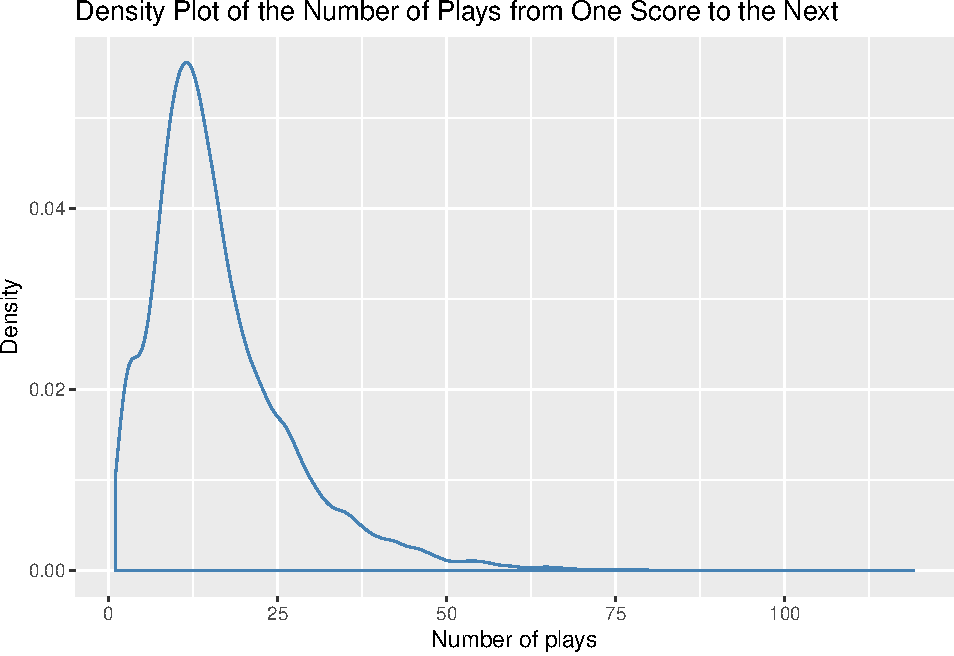
\includegraphics{thesis_files/figure-latex/test-log-norm-1.pdf}

To allow for more accurate sampling of the number of plays from the current game state to the next scoring play the ``fitdistrplus'' package by Marie-Laure Delignette-Muller is used to choose the parameters of a Log-Normal distribution that fit the data best. \(\sigma^{2}_{plays}\) is set to the variance parameter of the chosen Log-Normal and we sample:

\(log(plays_{i^*}) \sim \mathcal{N}(log(\hat{plays}_{i^*}),\sigma_{plays}^{2})\) so\\
\(plays_{i^*} = e^{log(plays_{i^*})}\)

To transform each sampled number of plays to time space we split the plays into plays that stopped the clock and plays where the clock continued to run.

\(nStopped_{i^*} \sim \mathcal{Binom}(plays_{i^*}, p_{stopped_{i^*}})\) and\\
\(nRunning_{i^*} = plays_{i^*} - nStopped_{i^*}\)

Where \(p_{stopped_{i^*}}\) is derived from a GBM detailed in the appendix. Draws that result in fewer than one clock stop are rejected because every scoring play stops the clock.

We next find the total time elapsed. We start by letting\\
\(K = nStopped_{i^*}\),\\
\(J = nRunning_{i^*}\),\\
\(S =\) time elapsed for a play after which the clock stops\\
\(R =\) time elapsed for a play after which the clock runs

\(S_{i^*_{1}}, \: S_{i^*_{2}}, \: ... , \: S_{i^*_{K}} \sim \mathcal{N}(\hat{S_i},\sigma_{S}^{2})\) where
\(\hat{S_i} = \beta_{int} + \beta_{down}down_i + \beta_{c_{score}}c_{score_i} + \beta_{ydstogo}ydstogo_i + \beta_{c_{score}down}c_{score_i}down_i\)

and

\(R_{i^*_{1}}, \: R_{i^*_{2}}, \: ... , \: R_{i^*_{J}} \sim \mathcal{N}(\hat{R_i},\sigma_{R}^{2})\) where
\(\hat{R_i} = \beta_{int} + \beta_{down}down_i + \beta_{c_{score}}c_{score_i} + \beta_{ydstogo}ydstogo_i + \beta_{c_{score}down}c_{score_i}down_i\)

We then find the time elapsed until the next scoring play as:\\
\(elapsed_{i^*} = \sum_{k=1}^{K}S_k + \sum_{j=1}^{J}R_j\)

Samples from \(\mathcal{N}(\hat{S_i},\sigma_{S}^{2})\) are rejected if they fall outside \([0, 15]\) and samples from \({N}(\hat{R_i},\sigma_{R}^{2})\) are rejected if they fall outside \([15, 50]\) in order to restrict sampled play lengths to a realistic distribution. Additionally, the entire process for sampling a particular value for time elapsed until the next scoring event is repeated if the sample causes an invalid game state\footnote{If a sample is rejected more than 10 times it is that the game state that will result in the end of the half and was misclassified} (i.e.~the time elapsed is greater than the amount of time remaining in the half).

Finally, the game states \(i^*_1, \:i^*_2, \:..., \: i^*_n \sim I^*\) are updated in accord with the values that have been sampled and we have:

\(WinProb_i = \frac{1}{n} \sum_{i^*}^{I^*}(WinProb_{i^*})\), where \(WinProb_{i^*}\) =

\(CDF^{-1}(\frac{\hat{\mu}_{i^*} + s_{curr_{i^*}}}{\sigma^{2}_{i^*}})\) for \(t_{i^*} > 600\),\\
\(GBM_{4th}(i^*)\) for \(t_{i^*}\) such that \(0 < t_{i^*} \leq 600\),\\
\(GBM_{ot}(i^*)\) for \(t_{i^*} < 0\)

\hypertarget{modeling-win-probability-in-other-scenarios}{%
\section{Modeling Win Probability in Other Scenarios}\label{modeling-win-probability-in-other-scenarios}}

When the game state does not fit any of the scenarios above\footnote{This will occur on any second, third, or fourth down play, as well as on first downs where there are more or less than ten yards to go}, it is first advanced to the next set of downs. To do this we take m samples of the triple (outcome of the current set of downs, time elapsed until the next set of downs, current set of downs results in scoring play). We also sample the number of yards downfield the ball will move over the current set of downs for all draws where the current set of downs does not result in a scoring play.

Seven possible outcomes are also defined for a given set of downs: conversion, turnover on downs, end half, field goal attempt, punt, safety, and turnover. As was the case when modeling the next scoring event, end of half, end of game, and overtime game states are modeled separately from other game states. Additionally, separate models were fit for each down because the log loss was lower for each down when separate models were fitted for each during LMRSO CV. End of half, end of game and overtime game states were all modeled with separate GBMs fit using the ``gbm'' package while all other game states were modeled with a multinomial logistic regression fit with the ``nnet'' package. The model formulas are listed in the appendix. The models all utilize down, yards to go, DVOA ratings, quarterback grades and a version of yard line that treats each 10 yard increment of the field as a separate group to help the model make better decisions about the likelihood of field goal attempts, punts, and fourth down conversion attempts.

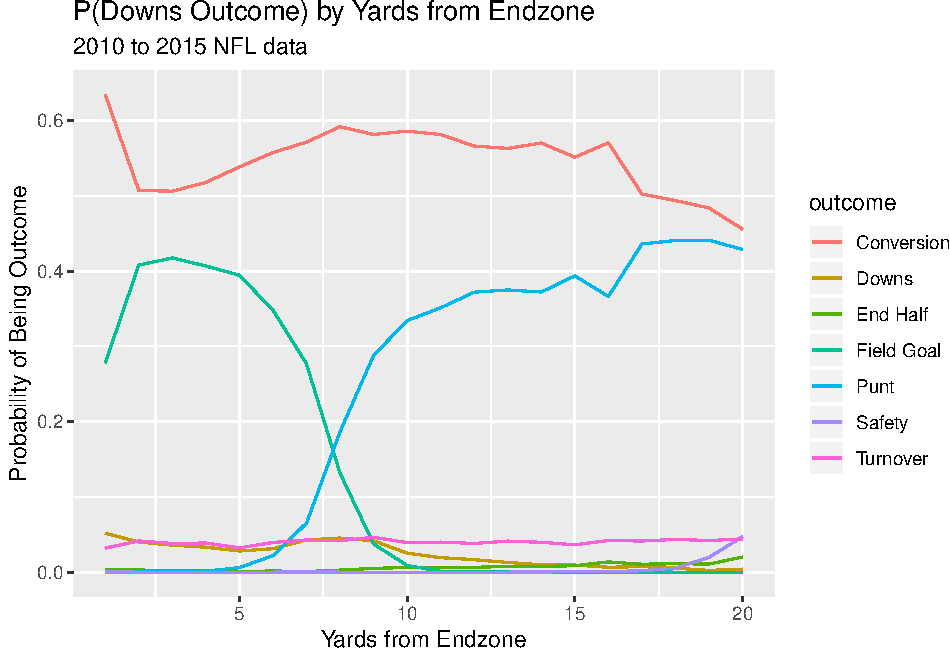
\includegraphics{thesis_files/figure-latex/fg-by-yardline-1.pdf}

After we have created a distribution \(\delta_i\) of potential outcomes of the set of downs associated with our inital game state \(i\) and sampled \(n\) outcomes \(outcome_{i^*_1}, \: outcome_{i^*_2}, \:..., \:outcome_{i^*_n} \sim \mathcal{Multinomial}(\delta_i)\), we move on to sampling from the distribution of time elapsed. We begin by sampling the number of plays until the next set of downs. This is treated as:

\(Plays_{i^*} = downstogo_{i^*} + replaysByPenalty_{i^*}\) where
\(downstogo_{i^*} = 5 - down_i\) for punts, turnovers on downs, and field goal attempts and\\
\(downstogo_{i^*} \sim \mathcal{Multinomial}(outcomeDist)\) for conversions, safeties, and turnovers where\\
\(outcomeDist =\)\\
\((0.349, 0.348, 0.276, 0.027)\) for conversions,\\
\((0.363, 0.312, 0.293, 0.032)\) for turnovers, and\\
\((0.333, 0.228, 0.272, 0.167)\) for safeties. Additionally,\\
\(replaysByPenalty_{i^*} \sim \mathcal{Binom}(downstogo_{i^*}, p_{penalty_i})\) where\\
\(p_{penalty_i}\) is taken from a GBM that predicts the probability of a given play being replayed due to penalty. It is listed in the appendix.

\(downstogo_{i^*}\) is set to be \(5 - down_i\) when \(outcome_{i^*}\) is a punt, turnover on downs or field goal attempt because those plays are assumed to happen only on fourth down. The multinomial distributions for conversions, turnovers and safeties simply refer to the probability that an outcome of the given type for a set of downs occurs on a given down. Samples from the distributions that imply the event happened on a down that has already occurred are rejected. Penalty replays refers to the number of plays until the next set of downs that will be replayed by penalty. To translate a sampled number of plays into time space we use the same equations and process that was detailed in section 2.2.

We next sample whether a given set of downs will result in a scoring play\footnote{All sets of downs where the sampled outcome is a safety are treated as scoring plays}.

\(score_{i^*} \sim \mathcal{Multinomial}(p_{fg_i}, p_{defTD_i}, p_{noScore_i})\) if \(outcome_{i^*} =\) fg attempt
\(score_{i^*} \sim \mathcal{Binomial}(p_{score_i} \: | \:outcome_{i^*})\) else

\(p_{score_i} | \:outcome_{i^*}\) is predicted by a GBM for sampled outcomes that are able to result in scores---conversions, field goals, punts and turnovers\footnote{Scores on conversions are assumed to be offensive touchdowns and scores on punts and turnovers are assumed to be defensive touchdowns}. Each GBM was fit using every set of downs that ended with the given outcome, and is listed in the appendix. For samples where score = 1 and the score is a touchdown, the game state is updated to include a draw for the point after that uses the same method outlined in the extra points sub-heading of 2.1. For these samples, as well as any samples where the \(outcome_{i^*}\) is the end of the half, we find that for each updated game\_state \(i^*\) the win probability is calculated in the same manner as it was in 2.2:

\(WinProb_{i^*}\) is:\\
\(CDF^{-1}(\frac{\hat{\mu}_{i^*} + s_{curr_{i^*}}}{\hat{\sigma}^{2}_{i^*}})\) for \(t_{i^*} > 600\),\\
\(GBM_{4th}(i^*)\) for \(t_{i^*}\) such that \(0 < t_{i^*} \leq 600\),\\
\(GBM_{ot}(i^*)\) for \(t_{i^*} < 0\)

For samples where score = 0 we must also sample a value for the number of yards downfield the ball will move over the current set of downs before calculating win probability. For each outcome other than conversions and field goal attempts\footnote{and end of halves where we don't need to sample this quantity at all}, two linear models are defined---one for downs first through third and one for fourth down---that specify a distribution for the number of yards downfield the ball will move for a given game state. Each linear model is listed in the appendix. The yards moved downfield is modeled separately for each possible outcome because doing so helped most of the linear models meet the assumption of constant residual variance and normally distributed errors\footnote{The exception to this is when the outcome of the set of downs is a conversion, but rejecting samples that were behind the first down marker alleviated this.}, allowing for easier sampling. The same reasoning is behind separating fourth down data from other data when fitting each model---the residual variance should be lower on fourth down for each outcome type because there is no longer uncertainty about where a punt, field goal attempt, etc. will be taken from. Conversions are a special case and are split into regular conversions and conversions by penalty.

\(ConversionType_{i^*} \sim \mathcal Bernoulli(p_{penaltyConv_i})\) if \(outcome_{i^*} =\) conversion

\(p_{penaltyConv_i}\) is defined by a logistic regression that has been trained on all conversion plays. The model only looked at the current down, the yards to go for a first and the interaction between the two variables. Yards moved downfield for conversions by penalty are also modeled with two linear models, one for fourth down and one for any other down. For regular conversions a linear model is specified for each down to better satisfy the linear regression constraints. Field goal attempts also work differently. Field goal attempts that don't result in a score are classified as either a regular miss or a block.

\(fgBlock_{i^*} \sim \mathcal Bernoulli(p_{block})\)

\(p_{block}\) is modeled using a GBM where the only predictors are yard line\footnote{Given a missed field goal, the shorter the attempt was, the more likely it was to be blocked} and down, where down likely only matters in the sense that it alerts the model as to whether the yard line might change between the current game state and any field goal try. The change in field position on regular field goal misses is modeled by a linear regression when the down is not fourth. On fourth down the ball is simply moved back 7 yards as is customary on missed field goals. Blocked field goals require the same protocol for determing change in field position as other possible outcomes. One linear model is used for downs first through third and another for fourth. For a given output \(\Delta\hat{fieldPosition}_i^*\) from the model \(m\) that is specified by \(outcome_{i^*}\) we take a sample:

\(\Delta fieldPosition_i^* \sim \mathcal N(\Delta\hat{fieldPosition}_i^*, \sigma^{2}_{\epsilon_m})\)

Samples drawn are rejected if they result in an invalid or illogical game state. Examples include first down conversions not by penalty where the draw would cause the game state to be short of the first down marker, a turnover on downs where the draw causes the ball to move past the first down marker, or any draw where the resulting game state features a yard line outside \([1, 99]\).

Once we have samples for the number of yards the ball has moved downfield we can fully update each of the game states for which a scoring outcome was not sampled. Each of these \(m \leq n\) remaining game states \(i^*_1, \: i^*_2, \:..., \:i^*_m \sim I^*\) will then go through the process outlined in 2.2. This will lead to the creation of \(M\) new game states \(j^*_1, \: j^*_2, \:..., \:j^*_M \sim J^* \:| \: i^*\)advanced from each game state \(i^*\) and will result in:

\(WinProb_{i^*} = \frac{1}{M}\sum_{j^*}^{J^*}WinProb_{j^* \: | \: i^*}\), where \(WinProb_{j^*} \: | \: i^*\) is:\\
\(CDF^{-1}(\frac{\hat{\mu}_{j*} + s_{curr_{j*}}}{\hat{\sigma}^{2}_{j*}}\:|\:i^*)\) for \(t_{j*}\:|\:i^* > 600\),\\
\(GBM_{4th}(j^*\:|\:i^*)\) for \(t_{j^*}\:|\:i^*\) such that \(0 < t_{j^*} \leq 600\),\\
\(GBM_{ot}(j^*\:|\:i^*)\) for \(t_{j^*}\:|\:i^* < 0\)

The resulting \(WinProb_i\) for the initial state \(i\) is then computed by taking averaging the values for of win probability for each game state \({i^*}\)\footnote{This includes the game states for which \(score{i^*}\) was equal to one and \(WinProb_{i^*}\) was calculated earlier.}:

\(WinProb_i = \frac{1}{n} \sum_{i^*}^{I^*}WinProb_{i^*}\)

\hypertarget{reasoning-behind-modeling-methodology}{%
\section{Reasoning Behind Modeling Methodology}\label{reasoning-behind-modeling-methodology}}

This methodology has several benefits. The first is that the impact of some game state descriptors like down, yards to go for a first down, and field position should theoretically be easier to measure on events they directly impact, like the outcome of a given set of downs, than on events they indirectly impact, like the probability of winning the game. Reducing noise around the measurement of the effects of game state descriptors like down, yards to go and yard line should improve model accuracy. Another benefit of modeling win probability like this is that it allows for a full distribution of EPA to be specified rather than a point estimate. This gives a better estimate of the variance associated with the game state which should lead to more accurate model predictions. Additionally, giving the model an estimate of the distribution of time that will elapse between the current game state and the next score gives the model an even fuller picture of the game and should help aid model accuracy, particularly towards the end of game. The modeling methodology also makes it easier to update the model piecemeal. If research comes out about the factors that influence the likelihood of converting a given set of downs, it shouldn't be very hard to incorporate the findings into the multinomial models that are currently in place to handle predicting the outcome of a given set of downs. It's also nice to get many of the benefits of a simulation without having to specify an exhaustive grid of conditional probabilities\footnote{Though this modeling protocol certainly comes with its fair share of edge cases to account for.}.

\hypertarget{results}{%
\chapter{Results}\label{results}}

Model performance is tested by re-training each sub-model on the entire training set\footnote{The training set is comprised of all the 2010-2016 data. During the tuning process each model was trained only on 2010-2015 data.} and evaluating the performance of the models when the protocol described in chapter 3 is used. Results are then are then compared against the other two models for which we have data---the models developed by Lock and Nettleton (2014) and Horowitz, Ventura, and Yurko (2018). The two loss functions used to measure model performance are Brier score, the mean of the squared distance between each prediction and the corresponding outcome, and log loss, the mean of the ln(1 - distance) for each prediction and the corresponding outcome.
\begin{longtable}[t]{lrrr}
\caption{\label{tab:resultsoverall}Brier score by model}\\
\toprule
  & Our Model & nflscrapR model & Lock and Nettleton model\\
\midrule
Brier score & 0.133 & 0.155 & 0.195\\
\bottomrule
\end{longtable}
\begin{longtable}[t]{lrrr}
\caption{\label{tab:resultsoverall}Log loss by model}\\
\toprule
  & Our Model & nflscrapR model & Lock and Nettleton model\\
\midrule
Log loss & -0.41 & -0.465 & -0.563\\
\bottomrule
\end{longtable}
We can also see that, as expected, the model generally performs better as the game progresses with the exception of overtime\footnote{There is a ceiling to how well even an all-knowing model could perform when predicting overtime because the games are so close to coin flips.}. Each model tested has a Brier score above 0.25 for the overtime period, indicating that, at least for the 2017 season, each model would be better off classifying every overtime game as a coin flip.
\begin{longtable}[t]{lrrrrr}
\caption{\label{tab:resultsquarter}Brier Score by Quarter}\\
\toprule
  & 1st Quarter & 2nd Quarter & 3rd Quarter & 4th Quarter & Overtime\\
\midrule
Our model & 0.183 & 0.156 & 0.112 & 0.081 & 0.255\\
nflscrapR model & 0.220 & 0.180 & 0.133 & 0.089 & 0.305\\
Lock and Nettleton Model & 0.303 & 0.229 & 0.163 & 0.097 & 0.480\\
\bottomrule
\end{longtable}
A plot has been included that omits overtime to show how average model performance improves over the course of games.

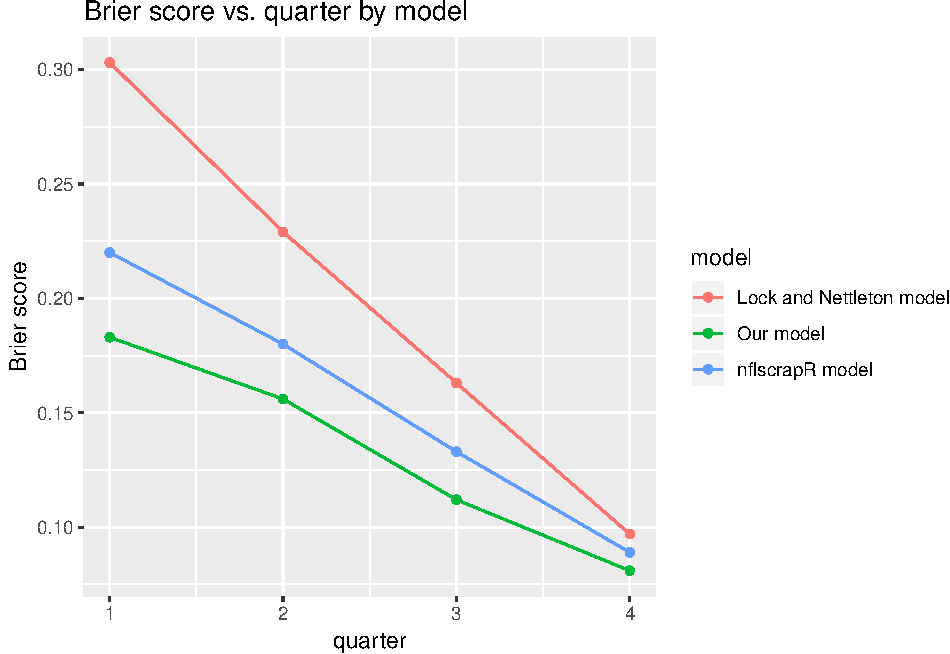
\includegraphics{thesis_files/figure-latex/resultsquarterplot-1.pdf}

The model also performs relatively evenly across each down (and kickoff and point after attempts), suggesting the predictions are mostly consistent.
\begin{longtable}[t]{lrrrrrr}
\caption{\label{tab:resultsdown}Brier Score by Down}\\
\toprule
  & 1st Down & 2nd Down & 3rd Down & 4th Down & Kickoff & Point After Attempt\\
\midrule
Our model & 0.133 & 0.134 & 0.133 & 0.129 & 0.130 & 0.130\\
nflscrapR model & 0.156 & 0.156 & 0.156 & 0.151 & 0.153 & 0.153\\
Lock and Nettleton Model & 0.196 & 0.196 & 0.196 & 0.191 & 0.194 & 0.195\\
\bottomrule
\end{longtable}
To test calibration game outcomes are grouped by bins that correspond to model predictions between a set of values. Twenty bins are created with each bin representing all points where the model predictions fell within a given five percent window. The mean game outcome is then plotted against the mean model prediction for each bin where the plot for a perfectly calibrated model would show a straight line with a slope of one.

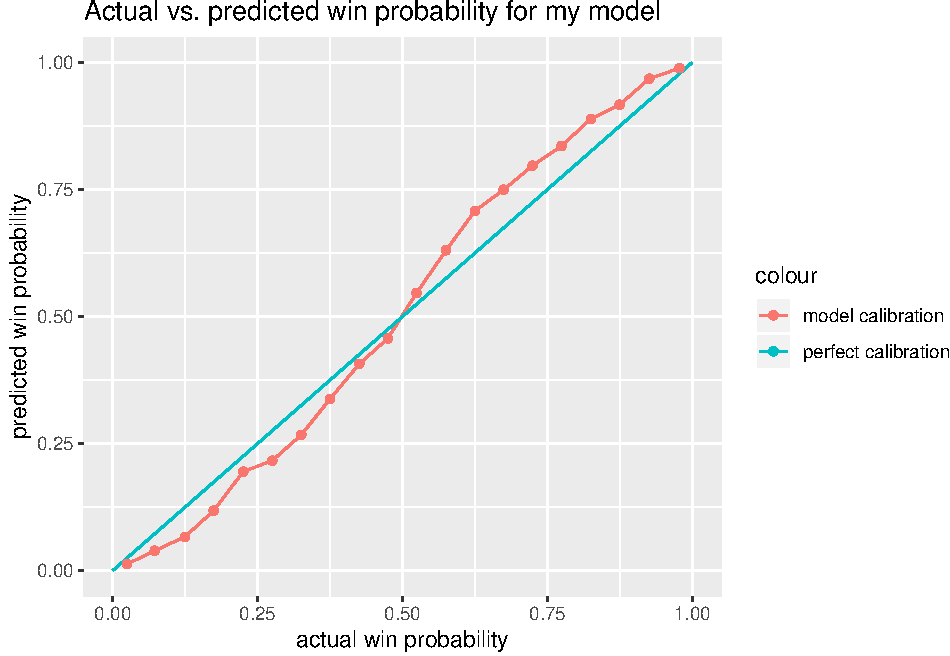
\includegraphics{thesis_files/figure-latex/calibration-1.pdf} 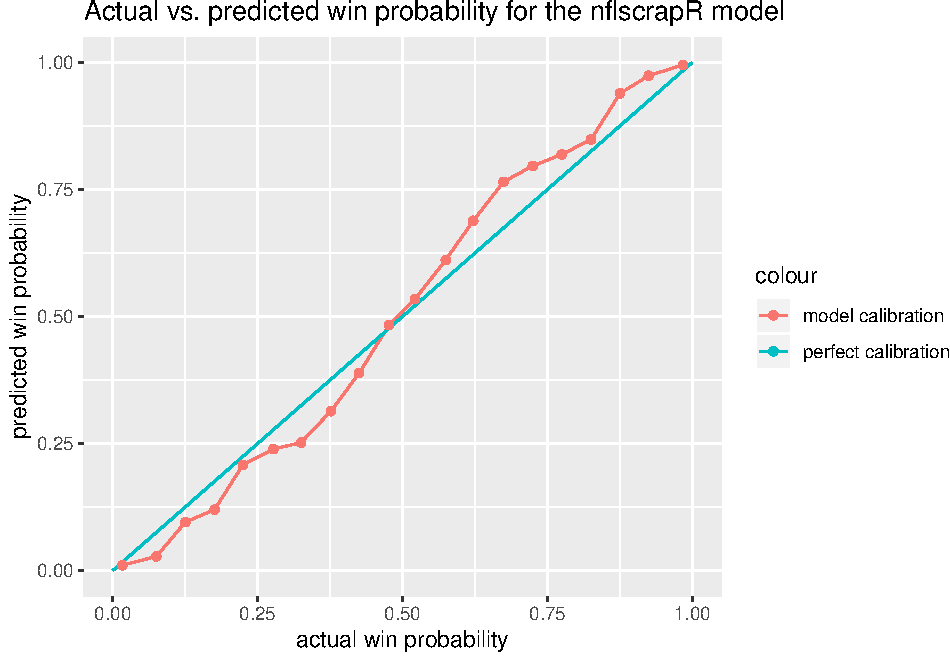
\includegraphics{thesis_files/figure-latex/calibration-2.pdf} 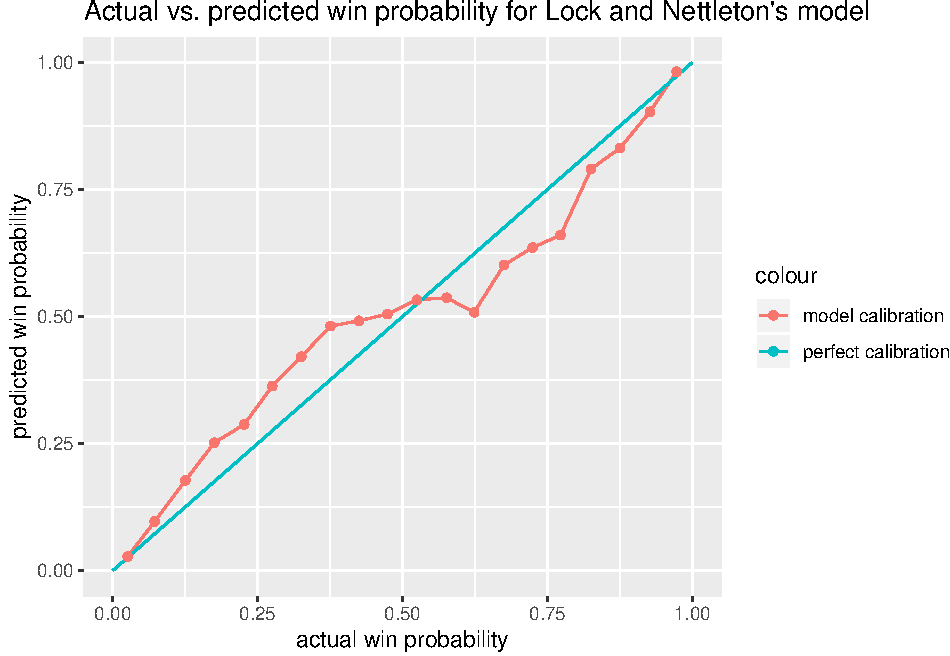
\includegraphics{thesis_files/figure-latex/calibration-3.pdf}

I was also curious whether model predictions become more accurate as the season progresses. It seems like the indicators of team strength included in the model---DVOA ratings and point spread---would become more precise as information about a team trickles in over the course of the season.

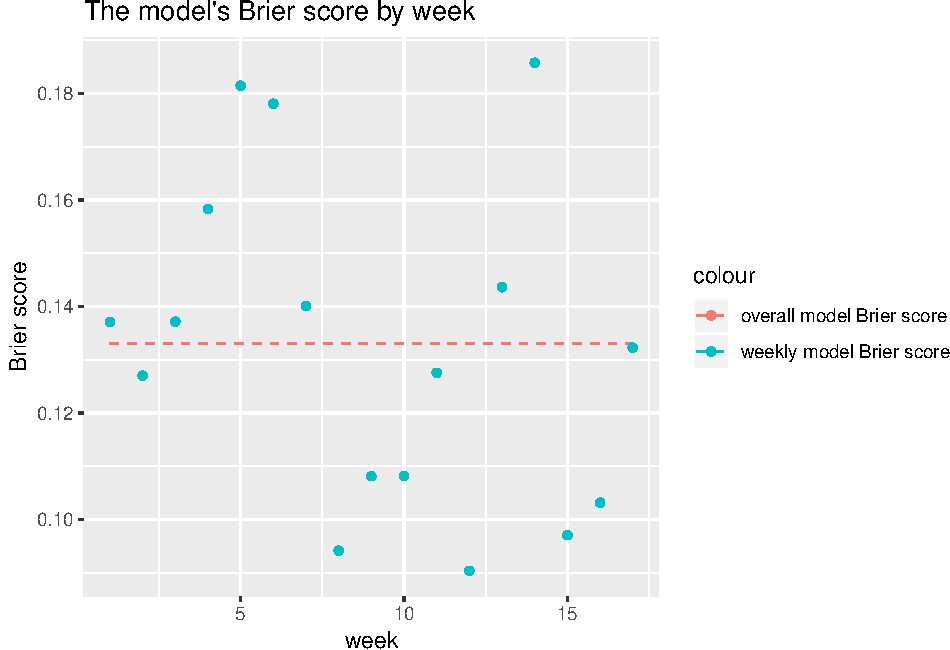
\includegraphics{thesis_files/figure-latex/resultsweekly-1.pdf}

The plot seems mostly random, but Brier score values did skew a bit lower as the season progressed. A linear regression of Brier score with week as a predictor found week to have a slope of -0.0018. This may be something to look at in the future.
\begin{verbatim}
Warning: Removed 8 rows containing missing values (geom_path).
\end{verbatim}
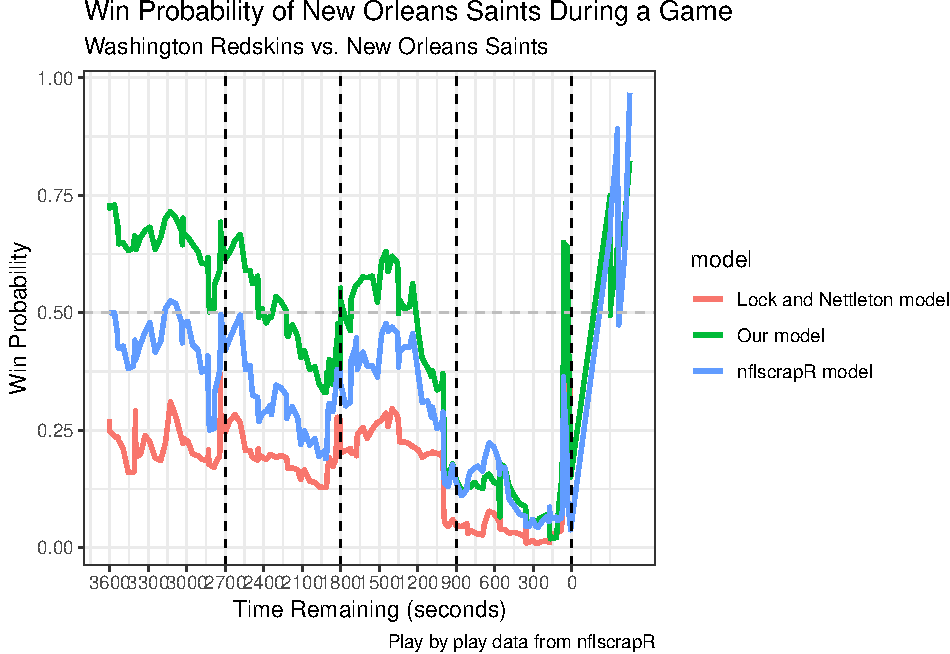
\includegraphics{thesis_files/figure-latex/examplegame-1.pdf}
In the game above, the Saints fell into an early hole before clawing back to force overtime on a touchdown with one minute left. They would win in overtime. This game seems instructive in terms of the strenghts of our model. We are more bullish on Saints winning than the other models from the get-go, likely because they were assumed by the model to be a much better team than the Redskins. Additionally, our model might be a bit more hesitant to shade too far towards teams that get out to early leads against a team with an offense like the Saints had in 2017, because of the increase in variance our model believes a potent offensive team to bring about.

\hypertarget{applications}{%
\chapter{Applications}\label{applications}}

This model has a variety of uses. It can be used by fans to improve their viewing experience---it's natural for a fan to be curious about his or her team's probability of winning during an NFL game. It can also be used to determine which plays contributed most to the outcome of the game.

Below is a graph of a 2017 regular season game between the Pittsburgh Steelers and Detroit Lions.

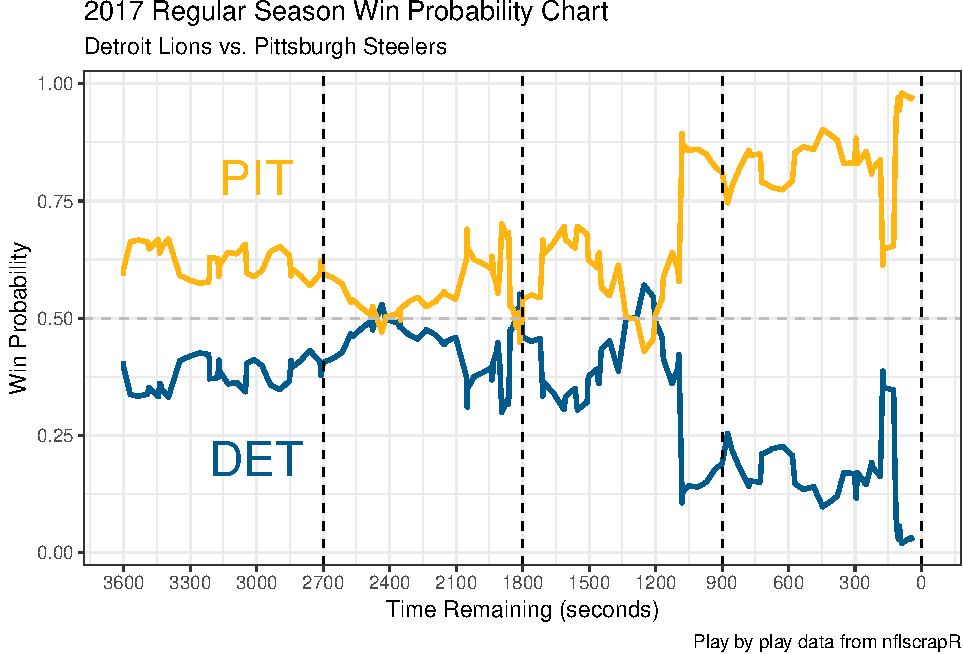
\includegraphics{thesis_files/figure-latex/examplegraph-1.pdf}

The Steelers would win the game 20-15, taking a 20-12 lead in the third quarter on a 97 yard touchdown pass from Ben Roethlisberger to Juju Smith-Schuster. We can find that this play boosted the Steelers chances of winning from 57.8\% to 87.1\%, a boost of 29.3\%. In fact, this play turns out to be the most impactful play of the goal. A 44 yard pass from Matthew Stafford to Eric Ebron to draw the Lions to the Pittsburgh 11 yard line with about three minutes remaining and the Lions down five was the only other play to swing the game more than 20\% (it checked in at a 22.5\% swing).

We can also use the model to evaluate coaching decisions, an application of win probability models that has been pioneered by Brian Burke (citation) and was also discussed by Lock and Nettleton (2014) and Horowitz, Ventura and Yurko (2018). During the game between Detroit and Pittsburgh detailed above, the Lions were down 13-12 midway through the third quarter and faced a 4th and goal from the Pittsburgh one yard line. Faced with a decision to attempt a field goal or go for a touchdown, the Lions opted to go for it. We can determine a breakeven point for the probability of scoring on the fourth down attempt that will make the value of a field goal attempt equal to that of going for it on fourth down. To do this we solve:

\(P_{score}*P(win \:|\: score)+(1-p_{score})* P(win \:| \: no \: score) =\)\\
\(p_{make} * P(win \:| \:make) + p_{miss} * P(win \:| \:miss)\)

Where \(p_{make}\) is calculated using the GBM discussed in 2.3 and the ball is assumed to be at the one yard line in the event of a failed fourth down attempt. We find that \(p_{score}\) must be greater than 37.0\% to justify going for it. The league average success rate on 2-point conversions is 47.9\%, and the Lions were at the one yard line, even closer than the two. They likely made the correct call.

Additionally, as Horowitz, Ventura, and Yurko (2018) show, player value can be derived by assigning credit to players on the field for fluctuations in win probability from one play to the next, though such an analysis is beyond the scope of this paper. The model might also be put to use to help determine when and in which direction to trade on prediction markets that deal with the probability of a given team winning an NFL game, though this application is also not investigated in this paper.

\hypertarget{discussion}{%
\chapter{Discussion}\label{discussion}}

Though the model performs well, it is not without its limitations. We model change in score using:

\(\Delta score_i \sim \mathcal{N}(\hat{\mu}_i,\hat{\sigma}^{2}_i)\) where
\(\hat{\mu}_i\) and \(\hat{\sigma}^{2}_i\) are defined in section 2.1.

But modeling \(\mu\) with a linear model assumes homoscedasticity, an assumption that is almost certainly incorrect. Additionally, none of the models account for different levels of uncertainty in the variables that describe team strength. It seems likely that the distribution of a team's possible DVOA ratings is much narrower at the end of the season than at the beginning. Ideally the model would reflect that. The model is also probably slightly off in certain situations where a specific outcome has not occurred in the data used to train the model. For example, there were not any safeties in overtime from 2010 to 2016 so the models used to predict the next scoring event or the outcome for a given set of downs will specify a probability of zero for a safety. While the probability of a safety in overtime is very low, it is not zero. Another model limitation can be found in the handling of field goal attempts, extra point attempts and two point conversions attempts where the probability of success is calculated using the league average success probability for each event as opposed to a model that takes into account the teams in question.

The model is also limited in the data it takes into account. Injuries to key players are not considered. Though the point spread is thought to take injuries into account, this still leaves the model blind both to in-game injuries and to the effects that injuries may have on the composition of a given team's strengths. The model also does not take weather into account. Generally this probably does not affect results much, but it would be nice to have a heads up when something extreme is happening in our dataset, like temperatures far below zero or snowstorms that verge on blizzards. The model also does not currently consider the strategic acumen of either coach, a factor that would seem to be important in close games. One last blind spot concerns timeouts, as the model currently does not consider them until ten or fewer minutes remain. Timeouts seem to help teams less by increasing the raw expectation of score differential and more by helping teams modify the distribution of discrete score differentials to their advantage at the end of games. As such, the choice was made not to include them in the linear models from which mu and sigma are taken.

\hypertarget{conclusion}{%
\section{Conclusion}\label{conclusion}}

By using a series of models to compute a distribution of EPA by sampling future game states, a variation of the trick PFR uses to derive win probability from the Normal CDF, and GBMs to handle win probability predictions when normality assumptions break down, the modeling process of this paper is able to achieve robust predictive results. Future versions of this model will ideally implement a form of heteroscedastic regression to better model the mu parameter as well as measures of uncertainty for predictors that stabilize over the course of a season. Future work may also be done to both quantify and include the effects of injury on win probability. Horowitz, Ventura, and Yurko (2018) detail a mechanism for applying the idea of ``wins above replacement'' (WAR), first developed in baseball, to the NFL. Such a measurement for NFL players would be very helpful for measuring the impact injuries might exert on win probability.

\appendix

\hypertarget{appendix}{%
\chapter{Appendix}\label{appendix}}

\hypertarget{qb-model}{%
\section{QB Model}\label{qb-model}}

A linear model was deemed sufficient for predicting a the PFF grade for a quarterback in a given seasons using past data. For a given quarterback and season combination \(i\), we have:

\(grade_{i} = \beta_{int} + \beta_{1}smoothGrades_i + \beta_{2}draftPick_i + \beta_{3}prevAttempts_i + \epsilon_i\)

where \(smoothGrades_i\) refers to a the weighted average of the grades a quarterback has received in previous seasons with more recent seasons weighted more heavily using a smooth exponential decay function with \(decay = 0.3\). A prior number of attempts of league average quarterback play was added to each grade outputted by the decay function. \(prior = 1500\) was chosen to minimize error through LMRSO CV.

\hypertarget{two-point-chart}{%
\section{Two Point Chart}\label{two-point-chart}}

The (very) naive two point decision making models assumes that teams go for two when the score differential is one of the following during the period between the touchdown and point after attempt:
\begin{longtable}{llllllllllll}
\toprule
  &  &  &  &  &  &  &  &  &  &  & \\
\midrule
Two Point Conversion Score Differentials & 19, & 12, & 5, & 4, & 1, & -2, & -9, & -10, & -16, & 17, & -18\\
\bottomrule
\end{longtable}
\hypertarget{clock-stop-gbm-to-predict-p_stopped}{%
\section{\texorpdfstring{Clock Stop GBM to Predict \(p_{stopped}\)}{Clock Stop GBM to Predict p\_\{stopped\}}}\label{clock-stop-gbm-to-predict-p_stopped}}

This GBM predicts the probability of the clock stopped on a given play by using the following variables where the value for each variable is the value for the variable at the previous kickoff to account for that face that this model has to predict the probability of the clock stopping not just for the current play but also for some number of plays in the future despite being unable to update other information.
\begin{longtable}[t]{l}
\caption{(\#tab:clockstop GBM)Variables used in GBM that predicts P(Clock Stoppage)}\\
\toprule
Variables\\
\midrule
Clock Will Stop\\
Number of Plays Until the Next Scoring Event\\
Timeout Adjusted Time Remaining in the Half\\
The Comeback Score\\
\bottomrule
\end{longtable}
\hypertarget{downs-outcome-formulas}{%
\section{Downs Outcome Formulas}\label{downs-outcome-formulas}}

For an initial game state \(i\), when \(t_i > 300\) \& !\((1800 < t_i <= 1980)\) a multinomial logistic regression model is fit, mimicking the process used to predict the next scoring event. The log odds \(\delta_ix\) for a given outcome \(x\) as compared to the baseline outcome are modeled by:

\(\delta_ix = \beta_{xint} +\beta_{xpos_{o}}pos_{o_i} + \beta_{xde\hspace{-0.1em}f_{o}}de\hspace{-0.1em}f_{d_i} +\beta_{xpos_{{qb}}}pos_{{qb}_i} + \beta_{xydstogo}ydstogo_i + \beta_{xyrd_{group}}yrd_{group_{i}}\)

Each GBM uses the following variables as well as a shrinkage parameter \(l = 0.02\), an interaction depth of two, and 1000 trees. The data on which they are trained is the only difference between the GBMs.
\begin{longtable}[t]{l}
\caption{(\#tab:downs gbms)Variables used in GBM that predicts P(Clock Stoppage)}\\
\toprule
Variables\\
\midrule
Offensive DVOA for the Team with the Ball\\
Defensive DVOA for the Team on Defense\\
Projected QB Grade for the Offensive Team\\
Yards to go for a First Down\\
Score Differential\\
\addlinespace
Timeout Adjusted Time Remaining in the Half\\
Yards from the End Zone Bucketed in Ten Yard Increments\\
\bottomrule
\end{longtable}
\hypertarget{gbm-for-p_penaltyreplay}{%
\section{\texorpdfstring{GBM for \(P_{penaltyReplay}\)}{GBM for P\_\{penaltyReplay\}}}\label{gbm-for-p_penaltyreplay}}

To output the probability of a penalty on a given play the GBM takes in the current down, the outcome of the set of downs and the field position of the offensive team. The shrinkage is given by \(l = 0.005\), the interaction depth is two and the number of trees is 1000.

\hypertarget{gbms-for-p_score}{%
\section{\texorpdfstring{GBMs for \(P_{score}\)}{GBMs for P\_\{score\}}}\label{gbms-for-p_score}}

The GBM that predicts \(P_{TD}\:| \:Conversion\) also uses a shrinkage parameter \(l = 0.02\), an interaction depth of two, and 1000 trees. It is fit with the following variables:
\begin{longtable}[t]{l}
\caption{\label{tab:off-td-gbm}Variables used in GBM that predicts P(Clock Stoppage)}\\
\toprule
Variables\\
\midrule
Offensive DVOA for the Team with the Ball\\
Defensive DVOA for the Team on Defense\\
Projected QB Grade for the Offensive Team\\
Yards to go for a First Down\\
Down\\
Yards from the End Zone\\
\bottomrule
\end{longtable}
The GBM that predicts \(P_{defTD}\:|\:Turnover\) utilizes a shrinkage parameter \(l = 0.02\), an interaction depth of two and 1000 trees. It is fitted with only three variables---the square root of yards from the end zone for the team punting, the offensive DVOA for the team on offense and the defensive DVOA for the team on defense.

The GBM that predicts \(P_{defTD}\:|\:Punt\) utilizes a shrinkage parameter \(l = 0.005\), an interaction depth of two and 1000 trees. It is fitted with only three variables---the yards from the end zone for the team punting and the special teams DVOAs for both teams.

The GBM that predicts \(P_{Make}\:|\:FG Attempt\) depends only on the square root of yards from the end zone for the team kicking the field goal, as does the GBM that predicts the \(P_{defTD}\:|\:FG Block\). Both have \(l = 0.01\) and \(ntrees = 1000\), though the field goal make GBM uses an interaction depth of one while the field goal block GBM uses an interaction depth of two.

\hypertarget{linear-models-for-delta-field-position-outcome_g}{%
\section{\texorpdfstring{Linear Models for \(\Delta field position | outcome_{g}\)}{Linear Models for \textbackslash{}Delta field position \textbar{} outcome\_\{g\}}}\label{linear-models-for-delta-field-position-outcome_g}}

\textbf{Conversion}\\
For first and second down all models for change in field position for conversions have the same formula. A given model \(m\) has formula as follows. A reminder that \(yrds\) is the field position of the offensive team:
\(y_{mi} = \beta_{mint} + \beta_{m1}ydstogo_i + \beta_{m2}\sqrt{yrds_i} + \beta_{m3}pos_{o_i} + \beta_{m4}def_{d_i} + \epsilon_{mi}\)

For third downs the model has formula:\\
\(y_{i} = \beta_{int} + \beta_{1}ydstogo_i + \beta_{2}\sqrt{yrds_i} + \beta_{3}pos_{qb_i} + \epsilon_i\)

and on fourth downs the model has formula:\\
\(y_{i} = \beta_{int} + \beta_{1}ydstogo_i + \beta_{2}\sqrt{yrds_i} + \beta_{3}pos_{o_i} + \epsilon_i\)

\textbf{Conversion by Penalty}\\
The model that handles first through third down has form:\\
\(y_{i} = \beta_{int} + \beta_{1}ydstogo_i + \beta_{2}\sqrt{yrds_i} + \beta_{3}down_i + \beta_{4}down_iydstogo_i + \epsilon_i\)

The model for fourth downs is:\\
\(y_{i} = \beta_{int} + \beta_{1}ydstogo_i + \beta_{2}\sqrt{yrds_i} + \epsilon_i\)

\textbf{Turnover on Downs}\\
The model for first through third down looks like:\\
\(y_{i} = \beta_{int} + \beta_{1}ydstogo_i + \beta_{2}\sqrt{yrds_i} + \beta_{3}pos_{qb_i} + \beta_{4}t_{adjH} + \beta_{5}t_{adjH}\sqrt{yrds_i} + \epsilon_i\)

The model for fourth downs is much simpler:\\
\(y_{i} = \beta_{int} + \beta_{1}ydstogo_i + \epsilon_i\)

\textbf{Punt}\\
The model for first through third down is:\\
\(y_{i} = \beta_{int} + \beta_{1}ydstogo_i + \beta_{2}\sqrt{yrds_i} + \beta_{3}pos_{st_i} + \beta_{4}def_{st_i} + \epsilon_i\)

The fourth down model is:\\
\(y_{i} = \beta_{int} + \beta_{1}\sqrt{yrds_i} + \beta_{2}pos_{st_i} + \beta_{3}def_{st_i} + \epsilon_i\)

\textbf{Turnover}\\
Though the field position change for turnovers is also modeled with separate models for fourth down and first through third down, the model formula is the same for both models (though coefficients are different). For a given model \(m\):

\(y_{mi} = \beta_{int} + \beta_{m1}ydstogo_i + \beta_{m2}\sqrt{yrds_i} + \beta_{m3}pos_{qb_i} + \epsilon_{mi}\)

\textbf{Field Goal}\\
The model for change in field position on missed field goals given the current down not being fourth is:\\
\(y_{i} = \beta_{int} + \beta_{1}ydstogo_i + \beta_{2}def_{d_i} + \beta_{3}down_i + \beta_{4}ydstogo_idown_i + \epsilon_{i}\)

For blocked field goals the model for change in field position on downs one through three is:\\
\(y_{i} = \beta_{int} + \beta_{1}ydstogo_i + \beta_{2}def_{d_i} + \beta_{3}\sqrt{yrds_i} + \epsilon_{i}\)

On fourth down the model is:\\
\(y_{i} = \beta_{int} + \beta_{1}\sqrt{yrds_i} + \epsilon_{i}\)

\backmatter

\hypertarget{references}{%
\chapter*{References}\label{references}}
\addcontentsline{toc}{chapter}{References}

\markboth{References}{References}

\noindent

\setlength{\parindent}{-0.20in}
\setlength{\leftskip}{0.20in}
\setlength{\parskip}{8pt}

\hypertarget{refs}{}
\leavevmode\hypertarget{ref-ESPN}{}%
Burke, B., \& Katz, S. (2017). How is total qbr calculated? We explain our quarterback rating. Retrieved from \url{http://www.espn.com/blog/statsinfo/post/_/id/123701/how-is-total-qbr-calculated-we-explain-our-quarterback-rating}

\leavevmode\hypertarget{ref-PFF}{}%
Eager, et a. (n.d.). PFF player grades. Retrieved from \url{https://www.profootballfocus.com/pff-player-grades}

\leavevmode\hypertarget{ref-friedman2001}{}%
Friedman, J. H. (2001). Greedy function approximation: A gradient boosting machine. \emph{Annals of Statistics}, \emph{29}(5), 1189--1232.

\leavevmode\hypertarget{ref-friedman2002}{}%
Friedman, J. H. (2002). Stochastic gradient boosting. \emph{Computational Statistics \& Data Analysis - Nonlinear Methods and Data Mining}, \emph{38}(4), 367--378.

\leavevmode\hypertarget{ref-lock2014}{}%
Lock, D., \& Nettleton, D. (2014). Using random forests to estimate win probability before each play of an nfl game. \emph{Journal of Quantitative Analysis in Sports}, \emph{10}(2), 197--206.

\leavevmode\hypertarget{ref-nflWAR}{}%
Maksim Horowitz, Samuel Ventura, \& Yurko, R. (2018). NflWAR: A reproducible method for offensive player evaluation in football. Retrieved from \url{https://arxiv.org/abs/1802.00998}

\leavevmode\hypertarget{ref-PFR}{}%
Neil Paine, et a. (n.d.). The p-f-r win probability model. Retrieved from \url{https://www.pro-football-reference.com/about/win_prob.htm}

\leavevmode\hypertarget{ref-FootballOutsiders}{}%
Schatz, et a. (n.d.). Methods to our madness. Retrieved from \url{https://www.footballoutsiders.com/info/methods\#DVOA}


% Index?

\end{document}
